\documentclass[12pt]{article} % Set base font size to 12pt
\usepackage{graphicx}
\usepackage{geometry} % Adjust page margins
\usepackage{setspace} % Line spacing
\usepackage{titlesec} % Customize section titles
\usepackage{tocloft} % Customize table of contents
\usepackage{fancyhdr} % Headers and footers
\usepackage{hyperref} % Add hyperlinks
\usepackage{xcolor} % Color package

% Set page margins
\geometry{a4paper, margin=2.5cm}

% Set line spacing
\setstretch{1.5} % Adjust line spacing for better readability

% Customize section titles
\titleformat{\section}[block]{\LARGE\bfseries\color{black}}{}{0em}{\filcenter}
\titlespacing*{\section}{0pt}{3.5ex plus 1ex minus .2ex}{2.3ex plus .2ex}

% Customize table of contents
\renewcommand{\cftsecleader}{\cftdotfill{\cftdotsep}}
\renewcommand{\contentsname}{Inhaltsverzeichnis}
\renewcommand{\cftaftertoctitle}{\par\nobreak\bigskip\bigskip\bigskip} % Add space after TOC title
\setlength{\cftbeforesecskip}{0.5em} % Adjust spacing between section entries
\setlength{\cftaftertoctitleskip}{2cm} % Adjust spacing between TOC title and entries
\hypersetup{
    colorlinks=true,
    linkcolor=blue,
    filecolor=magenta,
    urlcolor=cyan,
}

% Define headers and footers
\pagestyle{fancy}
\fancyhf{} % Clear default headers and footers
\fancyhead[R]{\thepage} % Page number on right side of header
\fancyhead[L]{\nouppercase{\leftmark}} % Chapter title on left side of header
\renewcommand{\headrulewidth}{0pt} % Remove header line
\fancyfoot[C]{\thepage} % Page number in the center of footer
\renewcommand{\footrulewidth}{0pt} % Remove footer line

% Define light gray color
\definecolor{lightgray}{RGB}{240,240,240}

\begin{document}

% Title Page
\begin{titlepage}
    \centering
    \vspace*{3cm}
    {\Huge\bfseries\textcolor{blue}{\MakeUppercase{ Cowboy Chaos: Eine humorvolle Wildwest-Geschichte }}\par} % Increased font size and colored title
    \vspace{0.5cm} % Adjust space between title and author
    {\Large\textit{ Maja Schmidt }\par} % Italic author name
    \vfill
    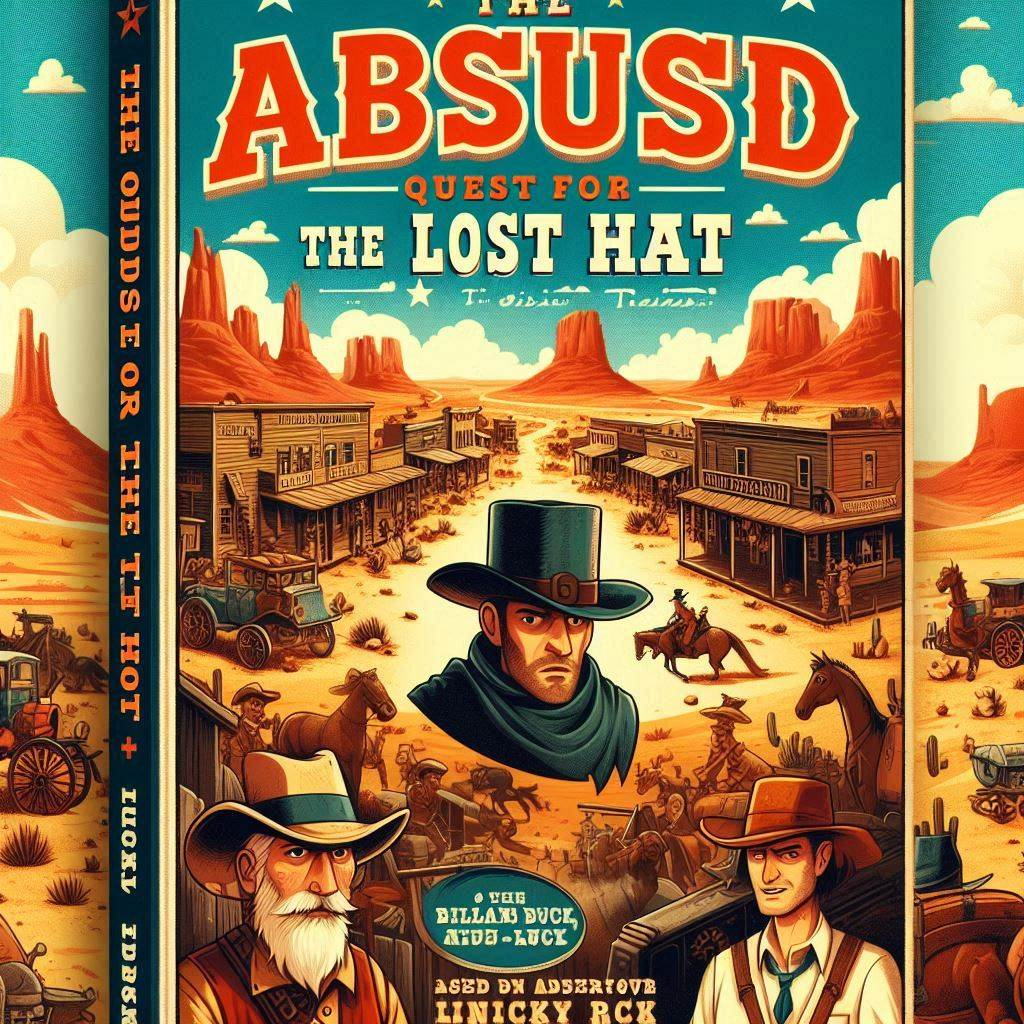
\includegraphics[width=0.9\textwidth]{ cover.jpg } % Larger cover image
    \vfill
    \today
\end{titlepage}

% Autorenvita
\section*{Autorenvita}
\vspace{4cm} % Adjust space between "Autorenvita" and "Inhaltsverzeichnis"
\begin{minipage}{\textwidth}
    Maja Schmidt ist eine renommierte Autorin, die sich auf humorvolle Western-Geschichten spezialisiert hat. Mit ihrem einzigartigen Schreibstil und ihrer Fähigkeit, das Western-Genre auf unterhaltsame Weise zu parodieren, hat sie bereits eine treue Leserschaft gewonnen. Ihre Bücher zeichnen sich durch eine gelungene Mischung aus Spannung, Charme und Humor aus, die die Leser immer wieder begeistert.
\end{minipage}

% Place table of contents on a separate page
\clearpage
\tableofcontents
\clearpage

% Chapters

\section{ Der verlorene Hut }
\begin{minipage}{\textwidth}
    Billy Buck, ein ungeschickter Cowboy mit einem Herzen aus Gold, stand auf dem staubigen Boden des Wilden Westens und spürte, wie ihm der Wind seinen geliebten Hut davontrug. Mit einem verzweifelten Aufschrei rannte er hinterher, doch der Hut tanzte wie von unsichtbarer Hand geleitet über die trockene Wüstenlandschaft. Billys unbeholfene Versuche, ihn zu fangen, endeten in einer Reihe absurder Missgeschicke, die ihn von einer komischen Situation in die nächste stolpern ließen. Als er sich schließlich erschöpft auf den Boden fallen ließ, tauchte plötzlich Lucky Lucy auf, die schlagfertige Saloon-Besitzerin mit einem Geheimnis. 'Na, Cowboy, scheint so, als hättest du ein Problem mit deinem Hut', sagte sie mit einem verschmitzten Lächeln. Billy, überrascht von ihrer unerwarteten Erscheinung, erzählte ihr von seinem verlorenen Hut und seiner absurden Suche. Lucky Lucy, die eine andere Seite des Wilden Westens repräsentierte, bot ihm ihre Hilfe an und gemeinsam begannen sie eine skurrile Reise, die sie in die lebhaften Städte und abgelegenen Ranches der fiktiven Wildwest-Kulisse führte. Auf ihrem Weg trafen sie auf skurrile Nebencharaktere und erlebten unerwartete Hindernisse, die zu humorvollen und spannenden Momenten führten. Doch Billys ungeschickte Natur und Luckys schlagfertiger Charme ließen sie jedes Hindernis überwinden, während sie sich langsam auf die große Enthüllung zubewegten, die ihre Geschichte in einem humorvollen und charmanten Abschluss enden ließ, der die Leser zum Lachen bringen würde.
\end{minipage}

\section{ Die ungewollte Verfolgungsjagd }
\begin{minipage}{\textwidth}
    Billy Buck rannte keuchend über die staubige Wildwest-Landschaft, die Sonne brannte heiß auf seinen Rücken. Sein geliebter Hut tanzte vor ihm her, als würde er sich über Billys verzweifelte Versuche, ihn zu fangen, lustig machen. 'Halt an, du elender Hut!', rief Billy außer Atem, während er über einen umgekippten Wassereimer stolperte und sich in einer Wolke aus Staub wiederfand. Plötzlich hörte er das Klappern von Pferdehufen und das Zischen einer Peitsche. Eine ungewollte Verfolgungsjagd begann, als Billy sich umdrehte und den berüchtigten Slick Rick auf seinem wilden Mustang heranrasen sah. 'Na, na, na, Billy Buck, auf der Flucht vor deinem eigenen Hut? Das ist ja lächerlich!', spottete Slick Rick mit einem fiesen Grinsen. Billy, der sich in einer absurden Situation wiederfand, versuchte verzweifelt, seinem unerwarteten Verfolger zu entkommen, während sein Hut weiterhin über die Landschaft wirbelte. Inmitten dieser skurrilen Verfolgungsjagd tauchte plötzlich Lucky Lucy auf, die mit einem gewagten Manöver Slick Ricks Pferd zum Stolpern brachte und Billy so die Möglichkeit zur Flucht verschaffte. 'Komm schon, Cowboy, wir müssen hier weg!', rief sie und schwang sich geschickt auf ihr eigenes Pferd. Gemeinsam galoppierten sie davon, verfolgt von Slick Rick, der sich geschworen hatte, Billy Buck zu demütigen. Die ungewollte Verfolgungsjagd führte sie durch die lebhaften Städte und abgelegenen Ranches, während sie sich neuen skurrilen Charakteren und unerwarteten Hindernissen stellen mussten. Doch Billys ungeschickte Natur und Luckys schlagfertiger Charme ließen sie jedes Hindernis überwinden, während sie sich langsam auf die große Enthüllung zubewegten, die ihre Geschichte in einem humorvollen und charmanten Abschluss enden ließ, der die Leser zum Lachen bringen würde.
\end{minipage}

\section{ Ein unerwarteter Verbündeter }
\begin{minipage}{\textwidth}
    Billy und Lucky Lucy setzten ihre abenteuerliche Reise fort, während sie sich durch die lebhaften Städte und abgelegenen Ranches der fiktiven Wildwest-Kulisse bewegten. Auf ihrer Suche nach Billys verlorenem Hut stießen sie auf immer skurrilere Hindernisse und unerwartete Charaktere. Eines Tages, als sie gerade dabei waren, einer wilden Büffelherde auszuweichen, hörten sie plötzlich das Klappern von Pferdehufen. Aus dem Staub tauchte ein ungewöhnlicher Verbündeter auf - ein alter, aber furchtloser Kauz namens Whiskey Joe. 'Ihr seid auf der Suche nach einem verlorenen Hut, nicht wahr?' fragte er mit einem verschmitzten Grinsen. 'Ich kenne da jemanden, der euch helfen könnte.' Billy und Lucky Lucy waren zunächst skeptisch, aber Whiskey Joe überzeugte sie mit seiner unkonventionellen Art und seinem beeindruckenden Wissen über die Wildwest-Landschaft. Gemeinsam machten sie sich auf den Weg zu einer geheimnisvollen Höhle, in der angeblich ein alter Hut-Sammler namens Mad Hatter lebte. Unterwegs teilte Whiskey Joe seine eigenen skurrilen Geschichten und Anekdoten, die Billy und Lucky Lucy zum Lachen brachten und ihre Reise noch abenteuerlicher gestalteten. Als sie schließlich die Höhle erreichten, wurden sie von einem exzentrischen Mann mit einem Turban und einem riesigen Bart empfangen. Mad Hatter hörte sich ihre Geschichte an und bot ihnen an, in seiner Sammlung nach Billys Hut zu suchen. Doch bevor sie das tun konnten, brach draußen ein gewaltiger Sandsturm los, der sie alle einsperrte. In der Enge der Höhle und mit der ungewissen Zukunft vor Augen, begannen die unerwarteten Verbündeten, sich besser kennenzulernen und sich aufeinander zu verlassen, während sie darauf warteten, dass sich der Sturm legte und sie ihre Suche fortsetzen konnten.
\end{minipage}

\section{ Die unerwartete Wende }
\begin{minipage}{\textwidth}
    Nachdem Billy und Lucky Lucy sich durch eine Reihe absurder Abenteuer und skurriler Situationen gekämpft hatten, fanden sie sich schließlich vor einer alten verlassenen Mine wieder. Es war an der Zeit, sich dem Geheimnis um Billys verlorenen Hut zu stellen. Plötzlich tauchte Slick Rick, der selbsternannte Revolverheld, auf und stellte sich ihnen in den Weg. 'Nun, nun, was haben wir denn hier? Der ungeschickte Billy Buck und seine schlagfertige Begleiterin auf der Suche nach einem alten Hut', spottete er mit einem fiesen Grinsen. Doch bevor er weitermachen konnte, wurde er von einem lauten Knall unterbrochen. Aus der Mine strömte Rauch, gefolgt von einer Gestalt, die keiner von ihnen erwartet hatte. Es war ein alter Mann, der sich als Billys verschollener Großvater entpuppte. Er hielt den verlorenen Hut in der Hand und lächelte verschmitzt. 'Es ist an der Zeit, dass du die Wahrheit erfährst, Billy', sagte er mit ernster Stimme. Was folgte, war eine Enthüllung, die alles, was sie zu wissen glaubten, auf den Kopf stellte. Slick Rick, der plötzlich nicht mehr so böse wirkte, offenbarte seine wahren Absichten und schloss sich unerwartet dem Team an. Gemeinsam entschlüsselten sie die Geheimnisse der Mine und fanden nicht nur Billys Hut, sondern auch einen Schatz, der ihr Leben für immer verändern sollte. Die absurden Abenteuer und überraschenden Wendungen führten zu einem humorvollen und charmanten Abschluss, der die Leser zum Lachen und Staunen brachte.
\end{minipage}

\clearpage
% Metadata
\section*{Metadaten}
\begin{minipage}{\textwidth}
    \colorbox{lightgray}{
        \begin{minipage}{\dimexpr\textwidth-2\fboxsep}
            \vspace{4cm}
            \begin{itemize}
                \item Name des Buches: Cowboy Chaos: Eine humorvolle Wildwest-Geschichte
                \item Name des Autors: Maja Schmidt
                \item Name des Herausgebers: Mark Zimmermann
                \item Name des Verlags: HdM AI Technologies
                \item Adresse des Verlags: Nobelstraße 10, 70569 Stuttgart
                \item Datum der Veröffentlichung: 2022-10-20
            \end{itemize}
            \vspace{4cm}
        \end{minipage}

    }
\end{minipage}


\end{document}